% Options for packages loaded elsewhere
\PassOptionsToPackage{unicode}{hyperref}
\PassOptionsToPackage{hyphens}{url}
%
\documentclass[
]{article}
\usepackage{lmodern}
\usepackage{amssymb,amsmath}
\usepackage{ifxetex,ifluatex}
\ifnum 0\ifxetex 1\fi\ifluatex 1\fi=0 % if pdftex
  \usepackage[T1]{fontenc}
  \usepackage[utf8]{inputenc}
  \usepackage{textcomp} % provide euro and other symbols
\else % if luatex or xetex
  \usepackage{unicode-math}
  \defaultfontfeatures{Scale=MatchLowercase}
  \defaultfontfeatures[\rmfamily]{Ligatures=TeX,Scale=1}
\fi
% Use upquote if available, for straight quotes in verbatim environments
\IfFileExists{upquote.sty}{\usepackage{upquote}}{}
\IfFileExists{microtype.sty}{% use microtype if available
  \usepackage[]{microtype}
  \UseMicrotypeSet[protrusion]{basicmath} % disable protrusion for tt fonts
}{}
\makeatletter
\@ifundefined{KOMAClassName}{% if non-KOMA class
  \IfFileExists{parskip.sty}{%
    \usepackage{parskip}
  }{% else
    \setlength{\parindent}{0pt}
    \setlength{\parskip}{6pt plus 2pt minus 1pt}}
}{% if KOMA class
  \KOMAoptions{parskip=half}}
\makeatother
\usepackage{xcolor}
\IfFileExists{xurl.sty}{\usepackage{xurl}}{} % add URL line breaks if available
\IfFileExists{bookmark.sty}{\usepackage{bookmark}}{\usepackage{hyperref}}
\hypersetup{
  pdftitle={linear norm plot},
  pdfauthor={Joshua},
  hidelinks,
  pdfcreator={LaTeX via pandoc}}
\urlstyle{same} % disable monospaced font for URLs
\usepackage[margin=1in]{geometry}
\usepackage{graphicx,grffile}
\makeatletter
\def\maxwidth{\ifdim\Gin@nat@width>\linewidth\linewidth\else\Gin@nat@width\fi}
\def\maxheight{\ifdim\Gin@nat@height>\textheight\textheight\else\Gin@nat@height\fi}
\makeatother
% Scale images if necessary, so that they will not overflow the page
% margins by default, and it is still possible to overwrite the defaults
% using explicit options in \includegraphics[width, height, ...]{}
\setkeys{Gin}{width=\maxwidth,height=\maxheight,keepaspectratio}
% Set default figure placement to htbp
\makeatletter
\def\fps@figure{htbp}
\makeatother
\setlength{\emergencystretch}{3em} % prevent overfull lines
\providecommand{\tightlist}{%
  \setlength{\itemsep}{0pt}\setlength{\parskip}{0pt}}
\setcounter{secnumdepth}{-\maxdimen} % remove section numbering
\usepackage{booktabs}
\usepackage{longtable}
\usepackage{array}
\usepackage{multirow}
\usepackage{wrapfig}
\usepackage{float}
\usepackage{colortbl}
\usepackage{pdflscape}
\usepackage{tabu}
\usepackage{threeparttable}
\usepackage{threeparttablex}
\usepackage[normalem]{ulem}
\usepackage{makecell}
\usepackage{xcolor}

\title{linear norm plot}
\author{Joshua}
\date{15/05/2020}

\begin{document}
\maketitle

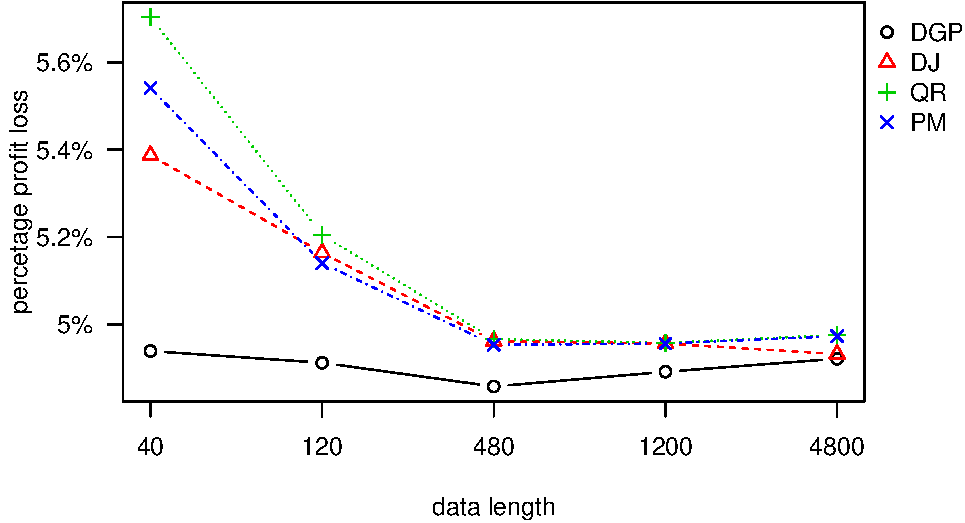
\includegraphics{linear-norm-plot_files/figure-latex/ppl0.5-1.pdf}

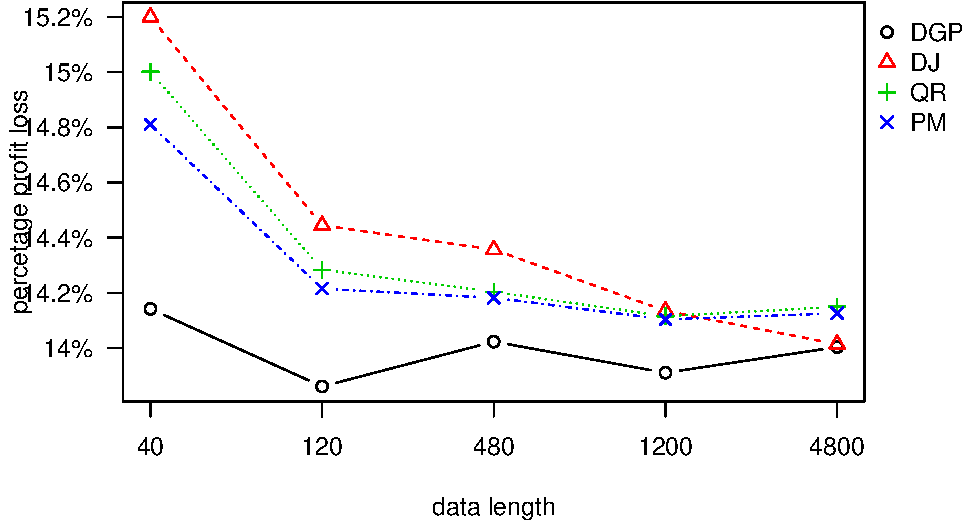
\includegraphics{linear-norm-plot_files/figure-latex/ppl0.63-1.pdf}

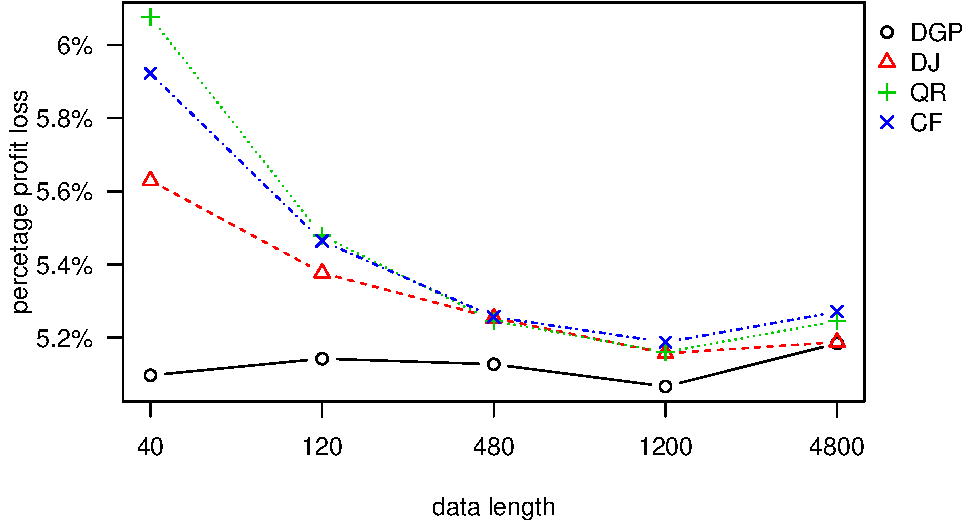
\includegraphics{linear-norm-plot_files/figure-latex/ppl0.3-1.pdf}

\begin{table}

\caption{\label{tab:inventory_error}Inventory Error}
\centering
\resizebox{\linewidth}{!}{
\begin{tabular}[t]{ccccccccccccc}
\toprule
\multicolumn{1}{c}{\textbf{ }} & \multicolumn{4}{c}{\textbf{Target service level=0.5}} & \multicolumn{4}{c}{\textbf{Target service level=0.63}} & \multicolumn{4}{c}{\textbf{Target service level=0.3}} \\
\cmidrule(l{3pt}r{3pt}){2-5} \cmidrule(l{3pt}r{3pt}){6-9} \cmidrule(l{3pt}r{3pt}){10-13}
Data size & DGP & disjoint & quantile & proposed & DGP & disjoint & quantile & proposed & DGP & disjoint & quantile & proposed\\
\midrule
\rowcolor{gray!6}  40 & -1.94 & 29.62 & -1.58 & -1.73 & -70.03 & -46.72 & -69.68 & -66.76 & 101.77 & 145.41 & 102.66 & 100.94\\
 & (200) & (221.78) & (217.24) & (214.91) & (199.58) & (221.15) & (217.92) & (215.23) & (198.78) & (220.78) & (219.04) & (216.5)\\
\rowcolor{gray!6}  120 & -0.34 & 11.59 & -0.67 & -0.62 & -69 & -61.58 & -69.06 & -67.86 & 107.02 & 126.82 & 107.01 & 105.56\\
 & (200.52) & (211.2) & (206.81) & (206.19) & (199.38) & (211.22) & (206.08) & (205.6) & (199.18) & (210.04) & (205.79) & (205.69)\\
\rowcolor{gray!6}  480 & -2.1 & 1.22 & -2.42 & -2.5 & -68.79 & -68.04 & -69.25 & -68.03 & 104.64 & 111.59 & 105.75 & 104.14\\
\addlinespace
 & (198.66) & (203.8) & (202.26) & (202.1) & (200.69) & (206.48) & (203.97) & (203.93) & (202.16) & (207.19) & (205.67) & (206.1)\\
\rowcolor{gray!6}  1200 & 3.65 & 5.61 & 3.22 & 3.25 & -67 & -67 & -67.54 & -66.4 & 103.87 & 107.71 & 104.55 & 103.06\\
 & (201.06) & (205.72) & (203.95) & (203.89) & (200.2) & (204.34) & (203.07) & (203.15) & (201.06) & (204.27) & (203.78) & (204.21)\\
\rowcolor{gray!6}  4800 & 0.41 & 0.81 & 0.84 & 0.86 & -68.34 & -68.09 & -69.22 & -68.08 & 102.76 & 103.43 & 104.18 & 102.76\\
 & (201.92) & (202.29) & (204.22) & (204.22) & (199.51) & (199.72) & (201.86) & (202.05) & (200.71) & (200.97) & (203.34) & (203.85)\\
\bottomrule
\end{tabular}}
\end{table}

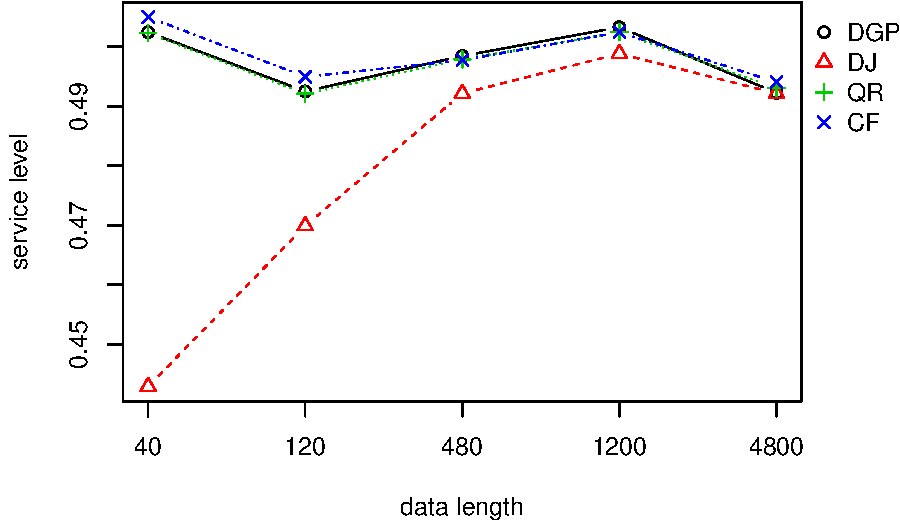
\includegraphics{linear-norm-plot_files/figure-latex/sl-1.pdf}
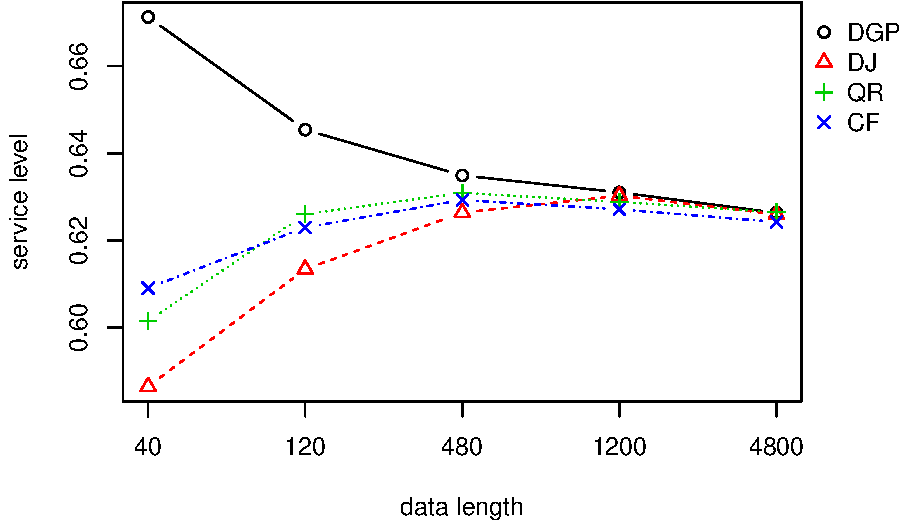
\includegraphics{linear-norm-plot_files/figure-latex/sl-2.pdf}
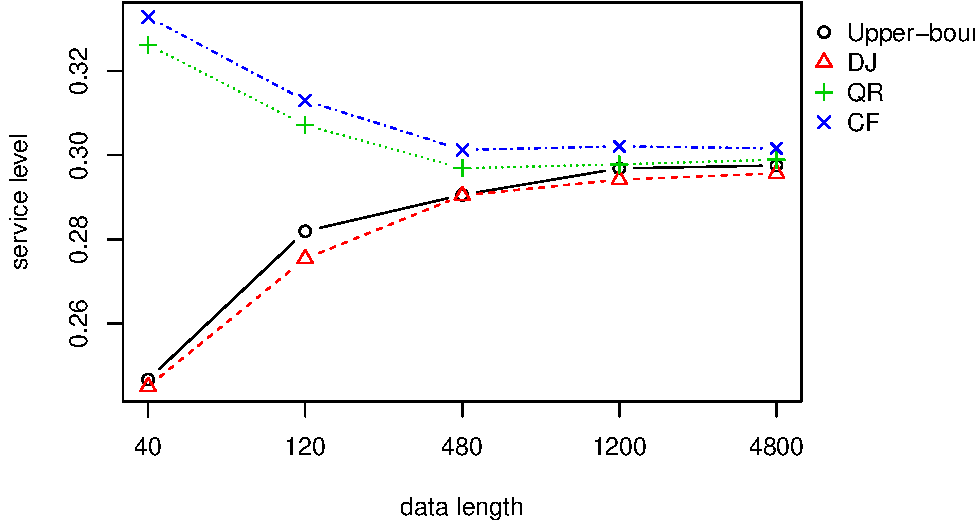
\includegraphics{linear-norm-plot_files/figure-latex/sl-3.pdf}
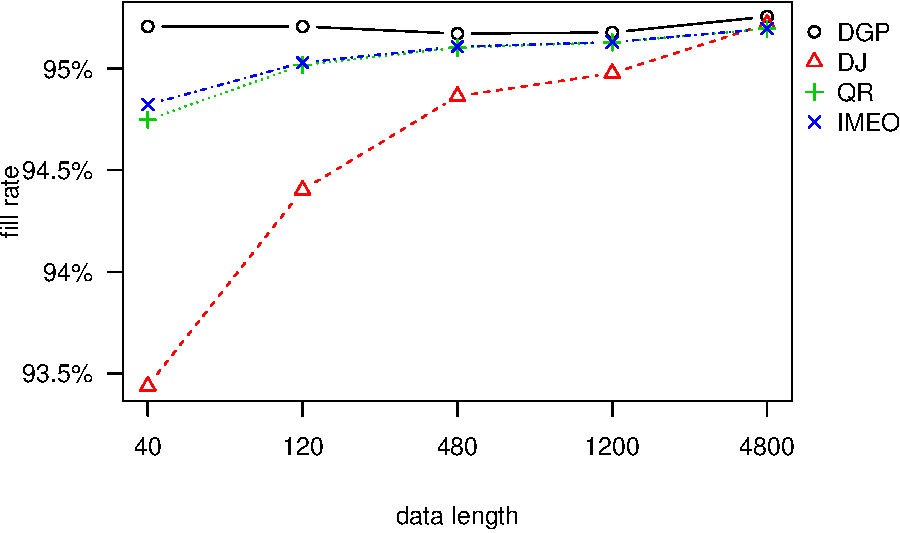
\includegraphics{linear-norm-plot_files/figure-latex/fr-1.pdf}
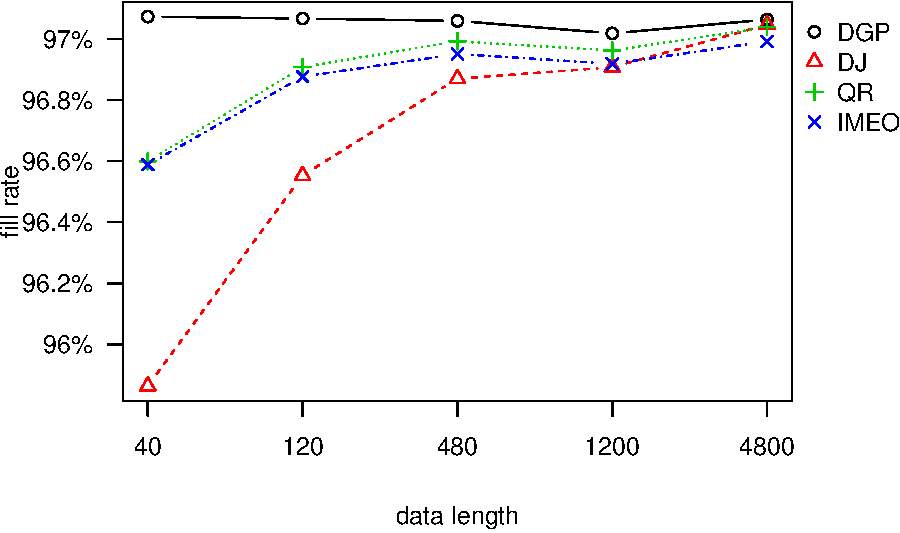
\includegraphics{linear-norm-plot_files/figure-latex/fr-2.pdf}
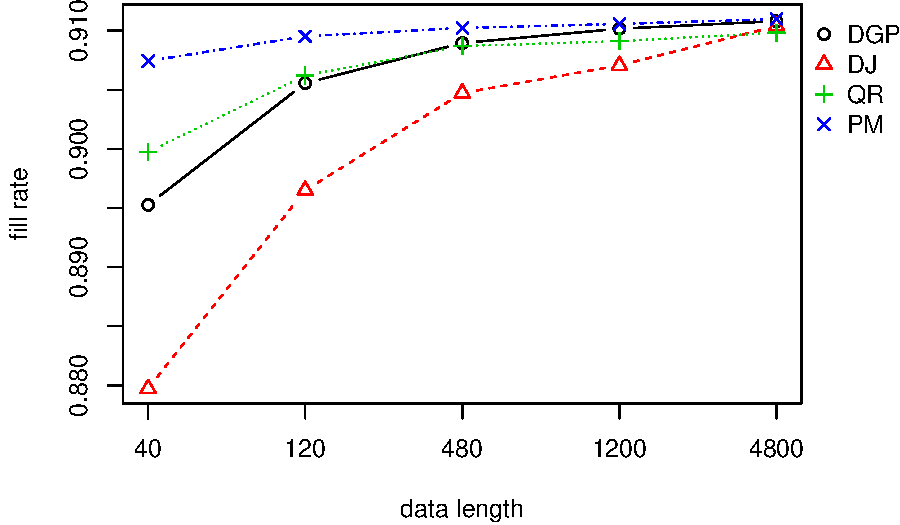
\includegraphics{linear-norm-plot_files/figure-latex/fr-3.pdf}

\begin{table}

\caption{\label{tab:Wilcoxon}p-value of Wilcoxon Test between data size 1200 and 4800}
\centering
\begin{tabular}[t]{ccccc}
\toprule
Target service level & DGP & disjoint & quantile & proposed\\
\midrule
\rowcolor{gray!6}  0.5 & 0.7641703 & 0.4008630 & 0.7489668 & 0.9282873\\
0.63 & 0.4873273 & 0.2296351 & 0.2332227 & 0.1992153\\
\rowcolor{gray!6}  0.3 & 0.6553228 & 0.3830332 & 0.8447936 & 0.6407884\\
\bottomrule
\end{tabular}
\end{table}

\begin{table}[H]
\centering
\resizebox{\linewidth}{!}{
\begin{tabular}{ccccccccccccc}
\toprule
\multicolumn{1}{c}{\textbf{ }} & \multicolumn{4}{c}{\textbf{Percentage profit loss}} & \multicolumn{4}{c}{\textbf{Service level}} & \multicolumn{4}{c}{\textbf{Fill rate}} \\
\cmidrule(l{3pt}r{3pt}){2-5} \cmidrule(l{3pt}r{3pt}){6-9} \cmidrule(l{3pt}r{3pt}){10-13}
Data size & DGP & DJ & QR & IMEO & DGP & DJ & QR & IMEO & DGP & DJ & QR & IMEO\\
\midrule
40 & 5.1\% & 5.6\% & 5.6\% & 5.6\% & 0.30 & 0.25 & 0.32 & 0.32 & 91.2\% & 88.4\% & 90.6\% & 90.8\%\\
120 & 5.1\% & 5.3\% & 5.3\% & 5.3\% & 0.29 & 0.27 & 0.30 & 0.30 & 91.0\% & 89.6\% & 90.8\% & 91.0\%\\
480 & 5.2\% & 5.3\% & 5.3\% & 5.3\% & 0.31 & 0.30 & 0.31 & 0.31 & 91.0\% & 90.5\% & 90.9\% & 91.0\%\\
1200 & 5.2\% & 5.3\% & 5.3\% & 5.3\% & 0.30 & 0.30 & 0.30 & 0.31 & 91.1\% & 90.8\% & 91.0\% & 91.1\%\\
4800 & 5.2\% & 5.2\% & 5.3\% & 5.3\% & 0.30 & 0.30 & 0.30 & 0.30 & 91.1\% & 91.1\% & 91.0\% & 91.1\%\\
\bottomrule
\end{tabular}}
\end{table}

\begin{table}[H]
\centering
\resizebox{\linewidth}{!}{
\begin{tabular}{ccccccccccccc}
\toprule
\multicolumn{1}{c}{\textbf{ }} & \multicolumn{4}{c}{\textbf{Percentage profit loss}} & \multicolumn{4}{c}{\textbf{Service level}} & \multicolumn{4}{c}{\textbf{Fill rate}} \\
\cmidrule(l{3pt}r{3pt}){2-5} \cmidrule(l{3pt}r{3pt}){6-9} \cmidrule(l{3pt}r{3pt}){10-13}
Target service level & DGP & DJ & QR & IMEO & DGP & DJ & QR & IMEO & DGP & DJ & QR & IMEO\\
\midrule
0.5 & 4.9\% & 5.4\% & 5.3\% & 5.3\% & 0.51 & 0.45 & 0.51 & 0.51 & 95.3\% & 93.4\% & 94.8\% & 94.8\%\\
0.63 & 13.9\% & 15.2\% & 15.1\% & 14.9\% & 0.64 & 0.58 & 0.63 & 0.63 & 97.1\% & 95.9\% & 96.6\% & 96.6\%\\
0.3 & 5.1\% & 5.6\% & 5.6\% & 5.6\% & 0.30 & 0.25 & 0.32 & 0.32 & 91.2\% & 88.4\% & 90.6\% & 90.8\%\\
\bottomrule
\end{tabular}}
\end{table}

\begin{table}[H]
\centering
\resizebox{\linewidth}{!}{
\begin{tabular}{ccccccccccccc}
\toprule
\multicolumn{1}{c}{\textbf{ }} & \multicolumn{4}{c}{\textbf{Percentage profit loss}} & \multicolumn{4}{c}{\textbf{Service level}} & \multicolumn{4}{c}{\textbf{Fill rate}} \\
\cmidrule(l{3pt}r{3pt}){2-5} \cmidrule(l{3pt}r{3pt}){6-9} \cmidrule(l{3pt}r{3pt}){10-13}
Target service level & DGP & DJ & QR & IMEO & DGP & DJ & QR & IMEO & DGP & DJ & QR & IMEO\\
\midrule
0.5 & 4.9\% & 5.0\% & 5.0\% & 5.0\% & 0.50 & 0.49 & 0.50 & 0.50 & 95.1\% & 95.1\% & 95.1\% & 95.1\%\\
0.63 & 13.8\% & 13.8\% & 14.0\% & 14.0\% & 0.63 & 0.63 & 0.63 & 0.63 & 97.1\% & 97.0\% & 97.0\% & 97.0\%\\
0.3 & 5.2\% & 5.2\% & 5.3\% & 5.3\% & 0.30 & 0.30 & 0.30 & 0.30 & 91.1\% & 91.1\% & 91.0\% & 91.1\%\\
\bottomrule
\end{tabular}}
\end{table}

\end{document}
